%==============================================================================
\section{Evaluation}
\label{sec:evaluation}
%==============================================================================

We evaluate \system against two state-of-the-art oblivious join baselines,
answering three questions:
\begin{enumerate}[leftmargin=*]
    \item How does \system compare against existing oblivious join approaches
    on multi-hop graph queries, across real and synthetic graphs of up to
    180M edges? (\cref{sec:evaluation:cross})
    \item Does \system generalize beyond chain queries to other join
    topologies such as fan-in, fan-out, and tree patterns?
    (\cref{sec:evaluation:shapes})
    \item Is \system's cost truly independent of the size of the unfiltered
    intermediate result, as promised by in-place filtering?
    (\cref{sec:evaluation:density})
\end{enumerate}

%------------------------------------------------------------------------------
\subsection{Experimental Setup}
\label{sec:evaluation:setup}
%------------------------------------------------------------------------------

All experiments run inside an Intel TDX guest VM on a recent Intel Xeon host,
with X vCPUs (X physical cores, 2-way SMT), 471 GB of RAM, and Ubuntu
24.04 (Linux 6.8). \sujaya{@Bish: State how much was used, not necessarily how much the machine supports.} By default, we run \system and its baseline with 64 threads.

\noindent\textbf{Baselines.}
We compare \system with:
\begin{itemize}[leftmargin=*]
    \item \textit{Full MWJ}: A system executing a graph query as an oblivious multi-way join (MWJ) using
    \wei \cite{ruidi2025oblivious} executed over the full, non-decomposed
    query, with predicate filtering applied after the join.
    \item \textit{Obliviator chained}: The state-of-the-art oblivious
    join scheme of Obliviator~\cite{mavrogiannakis2025obliviator}, applied
    hop-by-hop: each hop is an oblivious two-table join whose output is
    re-keyed and fed to the next hop.
    % We note that chaining two or more hops \textit{reveals
    % multiple intermediary result sizes}, making this baseline strictly weaker in
    % security for hops $>$1.

\end{itemize}

\begin{table}[t]
\centering
\caption{Leakage profile of the compared systems: which result sizes each
system reveals to an adversary observing memory. All systems reveal the
(public) input table sizes.}
\label{tab:leakage}
\begin{tabular}{lccc}
\toprule
 & \textbf{Hop-to-hop} & \textbf{Unfiltered} & \textbf{Filtered} \\
\textbf{System} & \textbf{intermediates} & \textbf{join output} & \textbf{output} \\
\midrule
Obliviator & revealed & revealed & revealed \\
Full MWJ & \textbf{hidden} & revealed & revealed \\
\system & \textbf{hidden} & \textbf{hidden} & revealed \\
\bottomrule
\end{tabular}
\end{table}

The three systems provide different security guarantees, summarized in
\Cref{tab:leakage}. Obliviator's chained execution materializes every
hop-to-hop intermediate join size at its true cardinality, which can be
a sensitive signal about graph structure. Full MWJ hides all intermediates inside the multi-way join, but must
materialize the \emph{unfiltered} join output before filtering, revealing
its size. \system reveals only the final \emph{filtered} output size as the
unfiltered intermediate is never materialized. \system therefore has
the strictest leakage profile of the three; where we nevertheless include
the leakier baselines, we are giving them the benefit of the doubt.

\smallskip
\noindent\textbf{Datasets.}
\Cref{tab:datasets} lists the six graph datasets we use in the evaluations.
\emph{Banking} is a synthetic
financial transaction graph produced by a seeded generator (1M accounts,
5M transactions, near-uniform degrees). The \emph{IBM AML} HI-Small, HI-Medium,
and HI-Large graphs are anti-money-laundering transaction networks from
IBM's AMLworld~\cite{altman2023realistic}; their degree
distributions are heavy-tailed, with hub accounts that participate in a
large fraction of transactions. \emph{LDBC SNB} is the person--knows--person
friendship graph of the LDBC Social Network Benchmark (Interactive
workload, scale factor 30)~\cite{erling2015ldbc}: a dense small-world
social network whose undirected friendships we mirror into directed edges,
giving an average degree of 73, an order of magnitude denser than the other
graphs. \emph{SNAP cit-Patents} is the US patent
citation network~\cite{snapnets}, a sparse citation DAG (average
out-degree 4.4).
% Besides node and edge counts, the table
% reports the number of \emph{unfiltered 2-hop paths},
% $\sum_a \mathit{in}(a)\cdot \mathit{out}(a)$ --- the size of the intermediate
% that a join-then-filter system must process for a 2-hop query. Skew
% decouples this quantity from edge count: Banking and HI-Small have the same
% number of edges, but HI-Small has $15\times$ more 2-hop paths; HI-Medium has
% $6\times$ more edges than cit-Patents but $146\times$ more paths.

\begin{table}[t]
\centering
\begin{tabular}{lrrr}
\toprule
\textbf{Dataset} & \textbf{Nodes} & \textbf{Edges} \\
\midrule
Banking (synthetic) & 1.0M & 5.0M \\
IBM AML HI-Small & 515K & 5.1M \\
LDBC SNB (SF30) & 165K & 12.0M \\
SNAP cit-Patents & 3.8M & 16.5M \\
IBM AML HI-Medium & 2.1M & 31.9M \\
IBM AML HI-Large & 2.1M & 179.7M \\
\bottomrule
\end{tabular}
\caption{Datasets.}
\label{tab:datasets}
\end{table}

\smallskip
\noindent\textbf{Queries.} We evaluate all three systems on multi-hop
queries, going up to X hops. Further, we evaluate \system on various join
patterns (chains, fan-in, fan-out, tree). When querying the synthetic
dataset, we leverage the query from \cref{sec:overview} mimicking a
fraud-detection query: starting from a flagged entity, follow $k$
node--edge--node hops and return the matching paths.
\system leverage the query decomposer to breakdown a query into on-hop
instances and construct a final residual query; baselines execute
the original query. The exact queries for each experiment can be
found in [].

\smallskip
\noindent\textbf{Reported timing.}
For each experiment, we report the time it took to execute a query.
We give each experiment a budget of one hour and the
full machine, and report runs exceeding the budget as timeouts (T/O) and
runs exhausting the 471 GB of memory as out-of-memory (OOM). Because many
experiments run for tens of minutes to hours, we report a single measured run per
cell, which we precede with a discarded warm-up run; repeated executions of
the faster experiments vary by at most $2\%$.
% We validate the output of every
% completing run against a plaintext SQLite baseline, and we additionally
% check output cardinalities against analytically computed ground truth.

%------------------------------------------------------------------------------
\subsection{Comparison on Real-world Datasets}
\label{sec:evaluation:cross}
%------------------------------------------------------------------------------

\begin{figure*}[t]
\centering
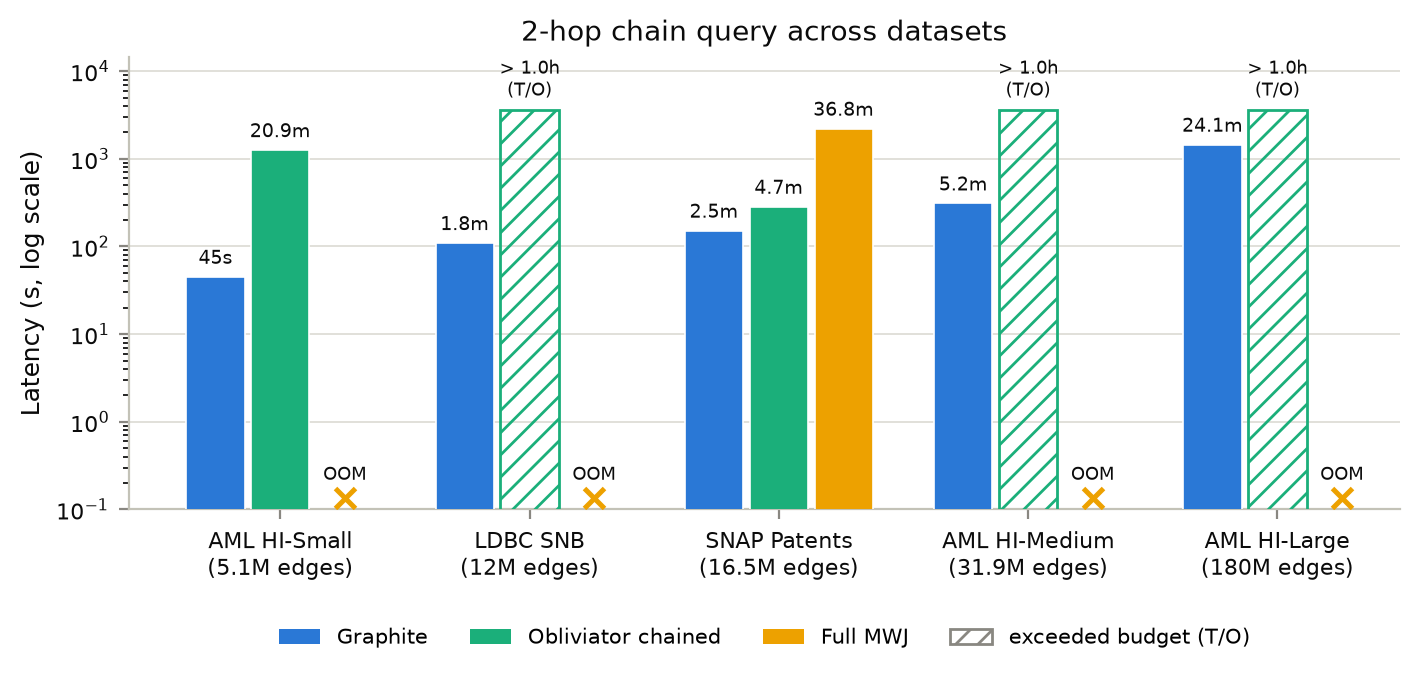
\includegraphics[width=0.65\textwidth]{figures/e3_cross_dataset.png}
\caption{A 2-hop query across five datasets (log-scale latency).}
\label{fig:cross_dataset}
\end{figure*}

\Cref{fig:cross_dataset} shows the result of comparing the three systems on
the five non-synthetic datasets, evaluated on a 2-hop query.

\system completes on every dataset, whereas each baseline completes on only
two of the five. Obliviator finishes HI-Small and cit-Patents but times out
on LDBC SNB (12M edges), HI-Medium, and HI-Large; Full MWJ completes only
cit-Patents and goes out-of-memory on the other four. On the datasets where a
baseline does complete, \system is $1.9$--$28\times$ faster than Obliviator
(which reveals intermediate sizes) and $14\times$ faster than Full MWJ on
the patent dataset. We note several counter-intuitive results: Obliviator takes
less time on the 16.5M-edge patent graph than on the 5.1M-edge HI-Small
graph; Full MWJ goes out-of-memory on the smaller HI-Small graph while
completing on the larger patent graph; and both baselines fail on the
12M-edge LDBC SNB graph while completing on the patent graph, which has
$1.4\times$ more edges. All of these occur because baseline cost is governed
by the size of the unfiltered intermediate join rather than the edge count.
The patent graph is sparse, so its 2-hop join produces 82.2M unfiltered
rows; HI-Small's hub accounts inflate its intermediate to 355.1M rows
despite a third of the edges; and SNB's uniformly high degree inflates it to
3.3B rows --- $40\times$ the patent graph's, from fewer edges. Notably, SNB
shows that this blowup does not require skewed hubs: on a dense graph,
\emph{every} node's in--out product is large. We study this effect in
detail in \cref{sec:evaluation:density}.

This experiment also highlights \system's scalability: as the graph grows
from the 16.5M-edge patent dataset to the 179.7M-edge AML HI-Large dataset,
\system smoothly handles the increase and completes the 2-hop query in
24.1 minutes, whereas Full MWJ runs out of memory. Despite revealing intermediary results,
even Obliviator fails on a 2-hop query on large inputs --- and, on the dense
SNB graph, already on a moderately sized one.




% These observations set up the remaining two experiments. Obliviator's
% chained kernel is a linear pipeline whose efficiency depends on
% revealing per-hop sizes; it supports only chain-shaped queries, and
% extending it to other topologies would require new kernels and yet more
% leakage. We therefore exclude it from the topology experiment and compare
% against the fully hiding Full MWJ (\cref{sec:evaluation:shapes}). Second,
% the correlation between baseline cost and intermediate size suggests that
% the unfiltered intermediate --- not the graph itself --- is what baselines
% pay for; \cref{sec:evaluation:density} isolates exactly this variable.

\subsection{Impact of Graph Density}
\label{sec:evaluation:density}
%------------------------------------------------------------------------------
\begin{figure}[t]
\centering
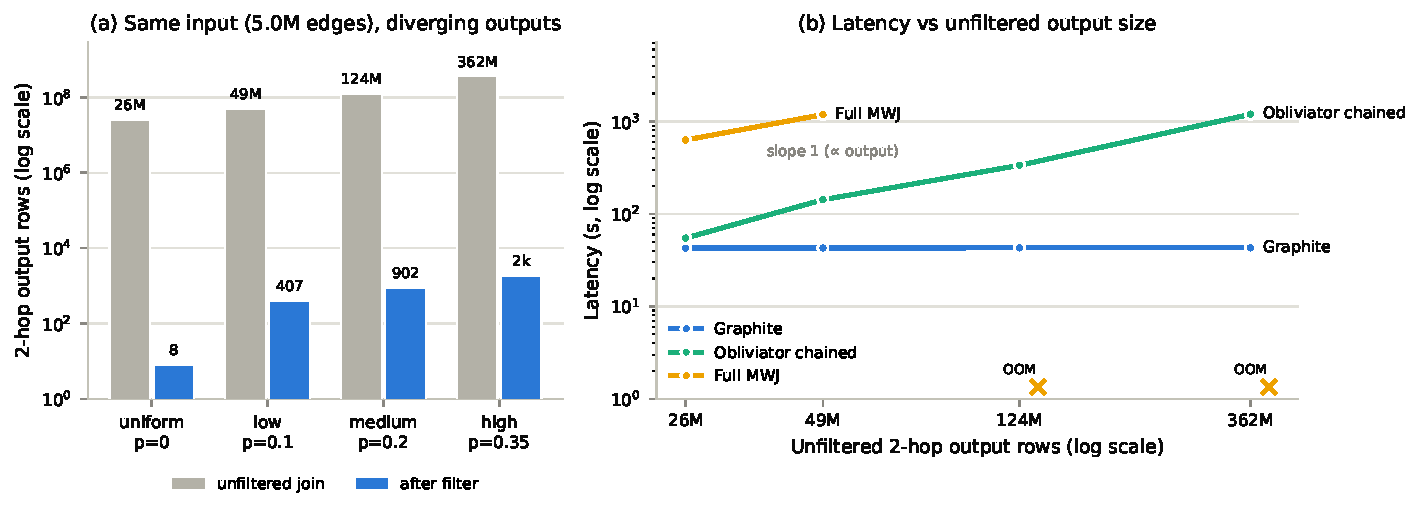
\includegraphics[width=\linewidth]{figures/e5_density_5M.png}
\caption{Impact of density on fixed-size inputs (1M nodes, 5M
edges). \system's latency remains roughly constant despite the unfiltered join
result size increasing from 29.1M to 362.1M rows due to increase in graph density,
which affects the baselines.}
\label{fig:density}
\end{figure}

The real-world dataset experiment hinted that graph density plays a vital
role in baseline performance, but it varied graph size, output size, and
density simultaneously. To isolate the effect of density alone, we use the
synthetic banking dataset and hold both the input size (1M accounts, 5M
transactions) and the final output size (under 2000 tuples) fixed. We
generate four variants that differ only in how edges concentrate on a
small set of hub accounts (hub fraction $p \in \{0, 0.1, 0.2, 0.35\}$).
Raising $p$ increases graph density directly, inflating the unfiltered
2-hop join from $26.1$M to $362.1$M rows as the graph becomes more
dense, producing a $13.9\times$ increase in join output size.

\Cref{fig:density} shows the results. Both baselines slow down as density
increases: Full MWJ's latency grows from 10.5 minutes at 26M unfiltered
rows to 19.7 minutes at 49M, then runs out of memory beyond 124M rows.
Obliviator degrades from 55 seconds to 19.9 minutes, a $21.8\times$
slowdown. \system, by contrast, holds latency flat at $42.7$--$43.1$s
across the experiment, despite the unfiltered
intermediate growing by $13.9\times$.

This experiment highlights two points. First, unlike the baselines, \system is
agnostic to density-driven blow-up in intermediate join size --- a
property especially valuable for property graph databases, where graph
structure routinely produces large intermediates even when the filtered
output stays small. Second, it provides empirical evidence for \system's
obliviousness guarantee: adversary-observable behavior should depend only
on public information, and since both input and output sizes are held
fixed here, \system's observable runtime remains unchanged too. The baselines, by
contrast, leak the graph's density through their running time alone.


%------------------------------------------------------------------------------
\subsection{Generality Across Query Topologies}
\label{sec:evaluation:shapes}
%------------------------------------------------------------------------------

Chain queries are only one traversal pattern. Analysts also ask
\emph{fan-in} queries (find $m$ distinct transactions converging on a
flagged account, a smurfing pattern), \emph{fan-out} queries ($m$
transactions leaving a flagged account, a dispersal pattern), and \emph{tree}
queries combining both. \system handles these topologies without
modification: the query decomposer turns \emph{every} edge of the join
graph into an independent \onehop operator regardless of shape, and only
the residual join structure changes. We run 2/3/4-hop chains plus a
fan-in, fan-out, and tree query, each with 4 edges, on AML HI-Small,
comparing \system against the baselines. We omit Obliviator on non-chain
queries because extending it beyond chains requires a non-trivial wrapper.

\begin{table*}[t]
\centering
\label{tab:shapes}
\begin{tabular}{lrrrrrr}
\toprule
\textbf{Query} & \textbf{Edges} & {\textbf{Unfiltered size}} & \textbf{Filtered size} & \textbf{\system} & \textbf{Full MWJ} & \textbf{Obliviator} \\
\midrule
1-hop & 1 & 5.1M & & & &\\
2-hop  & 2 & 355M & & 43\,s & OOM &\\
3-hop & 3 & 6.6B & & 84\,s & OOM &\\
4-hop & 4 & 134B & & 137\,s & OOM &\\
fan-in & 4 & 1.7T & 8M & 254\,s & OOM &\\
fan-out & 4 & $9.2{\times}10^{20}$ & 9.7M & 281\,s & OOM &\\
tree & 4 & $6.9{\times}10^{14}$ & 4.2M & 194\,s & OOM &\\
\bottomrule
\end{tabular}
\caption{Query topologies on AML HI-Small. ``Unfiltered rows'' is the
exact size of the intermediate a join-then-filter system must materialize.
Full MWJ exhausts the machine's RAM on every topology; Obliviator....}
\end{table*}

% \Cref{tab:shapes} shows the results. \system completes every topology in
% under five minutes, including the 4-edge star and tree patterns whose
% final outputs has millions of rows. Latency across the 4-edged queries varies
% only with the number of residual joins and the output size, not with the shape
% itself --- fan-in, fan-out, and
% tree each take within $1.4$--$2.1\times$ the latency of 4-edged
% chain. Full MWJ, by contrast, fails with out-of-memory on every topology,
% due to large unfiltered sizes.
% The ``unfiltered rows'' column explains why, and
% shows that this is not a memory-budget artifact: star and tree topologies
% compound hub degrees multiplicatively (fan-in over a node of in-degree $d$
% contributes $d^4$ rows), driving the unfiltered intermediate to $10^{12}$-$10^{20}$
% rows; the fan-out intermediate alone would occupy roughly
% $10^{23}$ bytes. Join-then-filter is therefore not merely slow on these topologies,
% it is infeasible at any practical scale.
% Shrinking the graph does not help, since
% even a 100$\times$ smaller banking graph (50K edges) still yields a
% $1.7{\times}10^{16}$-row fan-out intermediate. \system is unaffected by
% this blowup because it does not materialize the intermediate join, and its
% star and tree queries run in the same few minutes as the equally sized
% chain.

As shown in the last experiment, the latency of the baselines depends on unfiltered
intermediate rather than the graph's edge count or query's output size. Non-chain
topologies push this further: branching causes hub degrees to
\emph{compound multiplicatively} rather than accumulate additively along a
single path. A fan-in over a node of in-degree $d$ contributes $d^4$ rows
to the unfiltered join, versus a linear contribution for a chain of the
same length. This drives the unfiltered intermediate to $10^{12}$--$10^{20}$
rows for our 4-edge fan-in, fan-out, and tree queries --- the fan-out
intermediate alone would occupy roughly $10^{23}$ bytes, twelve orders of
magnitude beyond our 471GB RAM. The effect is structural, not an
artifact of graph size: even a 100$\times$ smaller banking graph (50K
edges) still yields a $1.7{\times}10^{16}$-row fan-out intermediate.
Join-then-filter is therefore not merely slow on these topologies; it is
infeasible at any practical scale, which is why Full MWJ goes out-of-memory
on every row of \cref{tab:shapes}.

\system is unaffected by this blowup, since it never materializes the
intermediate: \cref{tab:shapes} shows every topology completing in under
five minutes, including the fan-in, fan-out, and tree queries, whose
filtered outputs still run to millions of rows (8.0M, 9.7M, and 4.2M
respectively). Latency instead tracks the residual join structure and the
output size --- fan-in, fan-out, and tree each take within
$1.4$--$2.1\times$ the latency of the 4-hop chain, despite their unfiltered
sizes differing by up to eight orders of magnitude.

%------------------------------------------------------------------------------
\paragraph{Summary.}
Across all three experiments, the pattern is the same: the cost of prior
oblivious join approaches is governed by the size of intermediates they
materialize --- per-hop results for Obliviator, the unfiltered join for
Full MWJ --- and real graph workloads make those intermediates explode.
\system's costs are governed by the input size and the filtered output
size alone, which is why it completes every dataset, every topology, and
every density level in this evaluation, while leaking strictly less.
